% Manual de usuario de CEP. Compilar desde esta carpeta con:
%   pdflatex MANUAL_USUARIO.tex   (dos pasadas)
% Las imágenes están en img/ (capturas de la aplicación con los datos de demostración).
\documentclass[11pt,a4paper]{article}
\usepackage[T1]{fontenc}
\usepackage[utf8]{inputenc}
\usepackage{lmodern}
\usepackage[spanish,es-noshorthands,es-tabla,es-nodecimaldot]{babel}
\usepackage[margin=2.3cm,headheight=14pt]{geometry}
\usepackage{microtype}
\usepackage{amsmath,amssymb}
\usepackage{xcolor}
\usepackage{graphicx}
\usepackage{float}
\usepackage[font=small,labelfont=bf,skip=6pt]{caption}
\usepackage{booktabs,tabularx,array}
\usepackage{enumitem}
\usepackage{titlesec}
\usepackage{fancyhdr}
\usepackage{needspace}
\usepackage{tcolorbox}
\usepackage[hidelinks]{hyperref}

\definecolor{primario}{HTML}{0F4C5C}
\definecolor{gristexto}{HTML}{40484C}
\definecolor{fondo}{HTML}{EEF4F5}
\definecolor{borde}{HTML}{BFC8CB}
\definecolor{ambar}{HTML}{B45309}
\definecolor{fondoambar}{HTML}{FFF4E5}
\definecolor{verde}{HTML}{15803D}
\definecolor{rojo}{HTML}{B91C1C}
\definecolor{gris}{HTML}{70787C}

\titleformat{\section}{\needspace{8\baselineskip}\Large\bfseries\color{primario}}{\thesection.}{0.6em}{}
\titleformat{\subsection}{\needspace{6\baselineskip}\large\bfseries\color{primario}}{\thesubsection}{0.6em}{}
\titleformat{\subsubsection}{\needspace{5\baselineskip}\normalsize\bfseries}{}{0em}{}
\titlespacing*{\section}{0pt}{1.4em}{0.7em}
\titlespacing*{\subsection}{0pt}{1.2em}{0.5em}
\titlespacing*{\subsubsection}{0pt}{0.9em}{0.3em}

\setlength{\parindent}{0pt}
\setlength{\parskip}{0.55em}
\setlist{itemsep=0.2em,topsep=0.3em,leftmargin=1.5em}
\renewcommand{\arraystretch}{1.25}

\pagestyle{fancy}
\fancyhf{}
\fancyhead[L]{\small\color{gristexto}CEP — Control Estadístico de Procesos}
\fancyhead[R]{\small\color{gristexto}Manual de usuario}
\fancyfoot[C]{\small\thepage}
\renewcommand{\headrulewidth}{0.4pt}

% ---- Convenciones del manual
\newcommand{\boton}[1]{\textbf{#1}}                      % botón o enlace que se pulsa
\newcommand{\campo}[1]{«#1»}                             % nombre de un campo o texto en pantalla
\newcommand{\ruta}[2]{\textbf{#1}~$\rightarrow$~\textbf{#2}} % vista → pantalla
\newcommand{\bs}{\textbackslash{}}
\newcommand{\figura}[3]{% archivo, pie, ancho relativo
  \begin{figure}[!htbp]\centering
  \includegraphics[width=#3\linewidth,height=0.55\textheight,keepaspectratio]{img/#1}
  \caption{#2}\end{figure}}
\newtcolorbox{nota}[1][Nota]{colback=fondo,colframe=primario,boxrule=0.5pt,arc=2pt,
  left=6pt,right=6pt,top=4pt,bottom=4pt,fonttitle=\bfseries\small,title=#1,
  coltitle=white,before skip=8pt,after skip=8pt}
\newtcolorbox{cuidado}[1][Importante]{colback=fondoambar,colframe=ambar,boxrule=0.5pt,arc=2pt,
  left=6pt,right=6pt,top=4pt,bottom=4pt,fonttitle=\bfseries\small,title=#1,
  coltitle=white,before skip=8pt,after skip=8pt}
\newcolumntype{L}{>{\raggedright\arraybackslash}X}
\newcolumntype{P}[1]{>{\raggedright\arraybackslash}p{#1}}

\begin{document}

% ======================================================================= portada
\begin{titlepage}
\vspace*{2.5cm}
{\color{primario}\rule{\linewidth}{1.2pt}}\par\vspace{1.2em}
{\fontsize{30}{36}\selectfont\bfseries\color{primario} CEP\par}
\vspace{0.4em}
{\LARGE Control Estadístico de Procesos\par}
\vspace{1.5em}
{\Large Manual de usuario\par}
\vspace{1.2em}
{\color{primario}\rule{\linewidth}{1.2pt}}\par
\vspace{2em}
{\large Versión 1.0.0 \hfill Noviembre de 2026\par}
\vfill
\begin{minipage}{\linewidth}\color{gristexto}
Este manual explica, pantalla por pantalla, cómo usar CEP: cómo instalarlo, cómo registrar las
muestras de un proceso, cómo leer su estado y cómo hacer el análisis completo de control
estadístico, desde la carga de datos hasta el informe final.

\medskip
Está escrito para dos tipos de lectores: el \textbf{operario}, que registra las muestras en la
planta, y el \textbf{ingeniero o analista}, que configura el control y analiza los resultados. Los
capítulos 1 a 6 sirven a ambos; el capítulo 7 es para Ingeniería.

\medskip
Las imágenes muestran la aplicación con los datos de demostración que trae incorporados.
\end{minipage}
\end{titlepage}

{\setlength{\parskip}{0pt}\tableofcontents}
\newpage

% ======================================================================= 1
\section{Introducción}

\subsection{Qué es CEP}
CEP es un programa para vigilar la calidad de un proceso productivo con las herramientas del
control estadístico de procesos. En la planta se toman muestras periódicas (por ejemplo, cinco
envases cada 15 minutos) y se anotan sus mediciones o sus defectos. CEP guarda esas muestras, las
compara con el comportamiento habitual del proceso y avisa cuando algo cambia. Además calcula si el
proceso cumple con lo que exige el cliente y prepara informes para compartir los resultados.

Funciona en un solo computador, sin conexión a internet. Todos los datos quedan guardados en ese
equipo, en un único archivo de base de datos.

\subsection{Dos vistas para dos tipos de usuario}

\begin{tabularx}{\linewidth}{@{}P{2.6cm}P{4.2cm}L@{}}
\toprule
\textbf{Vista} & \textbf{Quién la usa} & \textbf{Para qué}\\
\midrule
\textbf{Operario} & Personal de planta & Registrar las muestras, ver en palabras simples cómo va el proceso, atender las alertas y reportar problemas.\\
\textbf{Ingeniería} & Ingeniero de calidad, analista o supervisor & Definir qué se controla, cargar datos, calcular y fijar los límites, analizar la capacidad, diseñar el plan de muestreo, configurar las reglas y emitir informes.\\
\bottomrule
\end{tabularx}

Se cambia de vista con los botones \boton{Operario} e \boton{Ingeniería} del encabezado. La vista
Operario no usa términos técnicos y su menú nunca lleva a pantallas de Ingeniería.

\subsection{Convenciones de este manual}
\begin{itemize}
\item Los botones y enlaces que se pulsan aparecen en \boton{negrita}.
\item Los textos que se ven en pantalla aparecen entre comillas: \campo{Guardar muestra}.
\item Una ruta como \ruta{Ingeniería}{Plantilla de carga} significa: elegir la vista Ingeniería y,
  en el menú de la izquierda, la pantalla Plantilla de carga.
\item Los números usan coma decimal (500,25), igual que en la aplicación.
\end{itemize}

% ======================================================================= 2
\section{Instalación y primer inicio}

\subsection{Requisitos}
\begin{itemize}
\item Windows 10 u 11 de 64 bits.
\item Microsoft Edge WebView2, que viene incluido en Windows 11 y en los Windows 10 actualizados.
\item Unos 205 MB de espacio libre.
\item Opcional: MiKTeX, para que los informes PDF se compilen con LaTeX. Sin él, la aplicación
  genera el PDF con un formato alternativo y lo avisa.
\end{itemize}

\subsection{Instalar}
\begin{enumerate}
\item Hacer doble clic en \texttt{CEP-Setup-1.0.0.exe}. La instalación es para el usuario actual
  y no pide permisos de administrador.
\item Si Windows muestra \campo{Windows protegió su PC}, pulsar \boton{Más información} y luego
  \boton{Ejecutar de todas formas}. El aviso aparece porque el instalador no tiene firma digital.
\item Seguir el asistente. Al terminar quedan un acceso directo en el escritorio y otro en el menú
  Inicio.
\end{enumerate}

\subsection{Abrir el programa}
CEP se abre en su propia ventana, sin navegador. La primera vez puede tardar hasta un minuto
mientras Windows revisa el programa; las siguientes, unos segundos (mientras tanto se ve una
pantalla de carga). Solo puede haber una ventana de CEP abierta: si se intenta abrir otra, aparece
el mensaje \campo{CEP ya está abierto en este equipo. Busca su ventana en la barra de tareas}.

Al cerrar la ventana se cierra el programa por completo.

\subsection{Primer inicio: la base está vacía}
La primera vez no hay procesos cargados y la aplicación lo indica con un aviso. Hay dos caminos:
\begin{itemize}
\item \textbf{Empezar con datos propios:} crear la primera variable en
  \ruta{Ingeniería}{Variables a controlar} (sección~\ref{sec:variables}) o directamente con la
  plantilla de carga (sección~\ref{sec:plantilla}).
\item \textbf{Explorar con datos de ejemplo:} en \ruta{Ingeniería}{Base de datos y respaldos},
  pulsar \boton{Cargar demostración}. Se cargan un proceso de envasado y los ejemplos del libro de
  Montgomery. Esta opción solo aparece con la base vacía.
\end{itemize}

\subsection{Dónde quedan los datos}
Todo se guarda en la carpeta \texttt{C:\bs Users\bs <usuario>\bs CEP\bs}, fuera de OneDrive:

\begin{tabularx}{\linewidth}{@{}P{3.4cm}L@{}}
\toprule
\textbf{Archivo o carpeta} & \textbf{Contenido}\\
\midrule
\texttt{cep.db} & La base de datos con todos los procesos, muestras, alertas e historial.\\
\texttt{reportes\bs} & Los informes PDF y Excel generados.\\
\texttt{respaldos\bs} & Copias de la base. Se hace una cada vez que se abre el programa y se conservan las últimas 20.\\
\texttt{registro.log} & Registro técnico de errores, útil para diagnosticar problemas.\\
\bottomrule
\end{tabularx}

Desinstalar el programa (Configuración de Windows $\rightarrow$ Aplicaciones) no borra esta carpeta.

% ======================================================================= 3
\section{Conceptos básicos}
Esta sección explica, sin fórmulas, las ideas que aparecen en todo el programa. El glosario del
final (sección~\ref{sec:glosario}) reúne las definiciones.

\begin{description}[style=nextline,leftmargin=1.5em,itemsep=0.4em]
\item[Proceso] La línea o máquina que se vigila, por ejemplo \campo{Línea de Envasado L-04}.
\item[Variable] La característica que se revisa en cada muestra. Puede ser una
  \textbf{medición} (un peso, un diámetro, una temperatura) o un \textbf{conteo} (cuántas unidades
  salieron malas, cuántas fallas tiene una pieza). Un proceso puede tener varias variables.
\item[Muestra] El grupo de unidades que se revisa cada cierto tiempo, por ejemplo 5 envases
  seguidos. En la parte técnica también se llama \emph{subgrupo}. Cada muestra tiene un número
  (\#1, \#2, \ldots) que no se repite.
\item[Tamaño de muestra y frecuencia] Cuántas unidades tiene cada muestra (\emph{n}) y cada cuánto
  se toma (por ejemplo, cada 15 minutos). Juntos forman el \emph{plan de muestreo}.
\item[Límites de control] El rango en el que varía el proceso cuando funciona como siempre. Los
  calcula la aplicación a partir de los datos. En las gráficas son las líneas rojas; entre ellas
  está la \emph{zona normal}.
\item[Valores aceptados (especificación)] Lo que exige el cliente, la norma o el plano: un mínimo,
  un máximo y un valor ideal. No los calcula la aplicación: los define el ingeniero. En las
  gráficas son las líneas grises punteadas.
\item[Fase I: conociendo el proceso] La etapa inicial. Se juntan entre 20 y 25 muestras, se
  calculan límites provisionales y se descartan las muestras afectadas por causas conocidas
  (un ajuste de máquina, un error de medición). Al terminar, el ingeniero \emph{congela} los
  límites.
\item[Fase II: monitoreo] Con los límites congelados, cada muestra nueva se compara con ellos. Si
  una muestra sale de la zona normal o aparece un patrón extraño, se genera una alerta.
\item[Reglas de detección] Los patrones que generan alertas: un punto fuera de los límites, varios
  puntos seguidos del mismo lado, una tendencia, etc. Se identifican con códigos (N1 a N8 y WE4),
  pero la vista Operario los explica siempre en palabras.
\end{description}

\subsection{Estado del proceso}
En todo momento el encabezado y la vista Operario muestran el estado del proceso con un color y
una frase:

\begin{tabularx}{\linewidth}{@{}P{2.2cm}P{4.2cm}L@{}}
\toprule
\textbf{Color} & \textbf{Lo que dice} & \textbf{Significado y qué hacer}\\
\midrule
\textcolor{verde}{\textbf{Verde}} & \campo{El proceso va bien} & Fase II sin alertas pendientes. Seguir tomando las muestras a tiempo.\\
\textcolor{ambar}{\textbf{Ámbar}} & \campo{Revisar} & Hay señales de que algo está cambiando. Revisar la alerta, observar la máquina y anotar lo encontrado.\\
\textcolor{rojo}{\textbf{Rojo}} & \campo{Detener y avisar} & El proceso se salió de lo normal (un punto fuera de los límites, valores muy cerca del límite, una parada o un lote retenido). Avisar al supervisor o al ingeniero antes de seguir.\\
\textcolor{gris}{\textbf{Gris}} & \campo{Conociendo el proceso} & Fase I: los límites son provisionales. Registrar las muestras como siempre.\\
\textcolor{gris}{\textbf{Gris}} & \campo{Sin datos} & La variable todavía no tiene muestras.\\
\bottomrule
\end{tabularx}

% ======================================================================= 4
\section{La pantalla de CEP}

\figura{op_general.png}{Pantalla principal de la vista Operario. Arriba, el encabezado; a la izquierda, el menú; en el centro, el contenido de la pantalla.}{1}

\subsection{Encabezado}
Está siempre visible y tiene, de izquierda a derecha:
\begin{itemize}
\item \textbf{Proceso y variable activos.} Al pulsarlo se despliega la lista de todas las variables
  de todos los procesos; la que se elige pasa a ser la variable de todas las pantallas. La lista
  también tiene la opción \boton{+ Nueva variable\ldots}. La aplicación recuerda la última
  variable elegida.
\item \textbf{Operario / Ingeniería}: cambia de vista.
\item \textbf{Turno y carta}: el turno en curso (por ejemplo \campo{Turno 2 | 14:00 - 22:00}) y,
  debajo, el tipo de carta, el tamaño de muestra y la fase de la variable activa.
\item \textbf{Estado del proceso}: el recuadro de color descrito en la sección anterior.
\item \textbf{Campana}: el número de alertas sin resolver. Al pulsarla se abre la pantalla de
  alertas.
\item \textbf{Usuario}: el nombre de quien está usando el programa. Al pulsarlo se puede cambiar.
  No hay contraseñas: el nombre sirve para dejar constancia de quién hizo cada registro. Si una
  acción necesita un nombre y no hay ninguno, la aplicación lo pide.
\end{itemize}

\subsection{Menú lateral}
Muestra las pantallas de la vista actual. Abajo tiene un recuadro de ayuda: en Operario,
\campo{Muestreo} (cada cuánto se toma la muestra, cuándo toca la próxima y un acceso directo a
\boton{Registrar muestra}); en Ingeniería, \campo{Tolerancias definidas} (valor ideal, mínimo,
máximo, tolerancia, tamaño de muestra y fase de la variable activa).

\subsection{Mensajes y ventanas de confirmación}
\begin{itemize}
\item Los resultados de cada acción aparecen como mensajes breves en la esquina inferior derecha
  (por ejemplo, \campo{Muestra \#26 guardada}). Los errores explican qué pasó y cómo corregirlo.
\item Las acciones importantes (congelar límites, excluir una muestra, restaurar un respaldo)
  abren una ventana de confirmación. Muchas piden un motivo, que queda guardado en el historial.
\end{itemize}

% ======================================================================= 5
\section{Recorrido recomendado}\label{sec:recorrido}
Este es el orden de trabajo típico para poner un proceso bajo control con CEP:

\begin{enumerate}[itemsep=0.45em]
\item \textbf{Definir qué se controla.} En \ruta{Ingeniería}{Variables a controlar}, crear el
  proceso y sus variables con el asistente: nombre, cómo se registra, tamaño de muestra,
  frecuencia y valores aceptados (sección~\ref{sec:variables}).
\item \textbf{Juntar las muestras de la Fase I.} Entre 20 y 25 muestras tomadas en condiciones
  normales. Se pueden cargar con la plantilla Excel (sección~\ref{sec:plantilla}), desde un archivo
  CSV (sección~\ref{sec:datos}) o registrarlas una a una en la vista Operario
  (sección~\ref{sec:registrar}).
\item \textbf{Revisar los supuestos.} En \ruta{Ingeniería}{Validación de supuestos}, comprobar que
  los datos se comportan como esperan las cartas (sección~\ref{sec:supuestos}).
\item \textbf{Estabilizar y congelar los límites.} En \ruta{Ingeniería}{Gráficos Variables} (o
  Atributos), revisar las cartas, excluir las muestras con causa conocida y pulsar
  \boton{Congelar límites} (sección~\ref{sec:graficos}).
\item \textbf{Evaluar la capacidad.} En \ruta{Ingeniería}{Capacidad}, ver si el proceso cumple
  la especificación (sección~\ref{sec:capacidad}).
\item \textbf{Ajustar el plan de muestreo.} En \ruta{Ingeniería}{Plan de muestreo}, elegir cuántas
  unidades revisar y cada cuánto (sección~\ref{sec:plan}).
\item \textbf{Monitorear.} En la vista Operario se registran las muestras nuevas y se atienden las
  alertas (sección~\ref{sec:operario}).
\item \textbf{Informar.} En \ruta{Ingeniería}{Reportes}, generar el informe PDF o el libro Excel
  (sección~\ref{sec:reportes}).
\end{enumerate}

% ======================================================================= 6
\section{Vista Operario}\label{sec:operario}
La vista Operario tiene cuatro pantallas: \boton{Registrar muestra}, \boton{Cómo va el proceso},
\boton{Alertas} e \boton{Historial de muestras}. Todas trabajan sobre la variable elegida en el
encabezado.

\subsection{Registrar muestra}\label{sec:registrar}
Es la pantalla de inicio. Se compone de cuatro partes.

\subsubsection{Estado y próxima muestra}
La franja superior repite el estado del proceso en grande, con la frase de qué hacer. A la derecha
indica cuándo toca la \campo{Próxima muestra}: una cuenta regresiva (por ejemplo \campo{03:42}),
\campo{¡Ahora!} cuando ya corresponde tomarla, o el aviso de que está atrasada. Debajo se ve el
número de la muestra que sigue y el plan (\campo{5 unidades cada 15 min}). El botón
\boton{Reportar un problema} está explicado en la sección~\ref{sec:problema}.

\subsubsection{Cómo registrar una muestra}
\begin{enumerate}
\item Tomar las unidades indicadas (por ejemplo, 5 unidades seguidas) y medirlas.
\item Escribir el valor de cada unidad en \campo{Unidad 1}, \campo{Unidad 2}, etc. Se acepta coma
  o punto decimal. La tecla \textbf{Enter} pasa al campo siguiente.

  Si la variable es un conteo, el formulario pide en su lugar cuántas unidades se revisaron y
  cuántas salieron defectuosas (o cuántas fallas se encontraron).
\item Mientras se escribe, aparece debajo el \textbf{resultado en vivo}: el promedio de la muestra,
  si está dentro de lo normal y cuántas unidades quedaron fuera de los valores aceptados.
\item Opcionalmente, escribir el \campo{Lote}.
\item Pulsar \boton{Guardar muestra}.
\end{enumerate}

Si la muestra queda fuera de lo normal, al guardarla se crea una alerta y el estado del proceso
cambia de color.

\figura{op_sospechoso.png}{Aviso de valor probablemente mal escrito: 5000 en lugar de 500,0.}{0.85}

\textbf{Valores sospechosos.} Si un valor está muy lejos de lo habitual (por ejemplo 5000 en lugar
de 500,0), antes de guardar aparece la pregunta \campo{¿Están bien escritos estos valores?}. Con
\boton{Corregir} se vuelve al formulario; con \boton{Sí, están bien} se guarda igual.

\subsubsection{Deshacer la última muestra}
Durante los 10 minutos siguientes a guardar una muestra aparece el recuadro \campo{¿Te equivocaste
en la muestra \#25? Puedes deshacerla durante 09:25} con el botón \boton{Deshacer}. Al usarlo:
\begin{itemize}
\item se pide un motivo opcional (por ejemplo \campo{Error al escribir un valor});
\item la muestra no se borra: queda marcada como \emph{anulada} en el historial, con el motivo;
\item sus valores vuelven al formulario para corregirlos y guardarlos de nuevo.
\end{itemize}

\subsubsection{Gráfica y resumen}
A la derecha del formulario, la gráfica \campo{Últimas muestras} muestra el promedio de cada una
de las últimas 25 muestras con la zona normal sombreada. Debajo, tres recuadros resumen: el
porcentaje de unidades dentro de lo aceptado, el promedio frente al valor ideal y cuántas muestras
hay para revisar. \boton{Ver más detalle} abre la pantalla \emph{Cómo va el proceso}.

\figura{op_alertas_turno.png}{Alertas del turno y resumen del turno, en la parte inferior de la pantalla Registrar muestra.}{0.85}

\subsubsection{Alertas del turno y resumen del turno}
Más abajo están las \campo{Alertas del turno}, cada una explicada en palabras y con el botón
\boton{Anotar qué pasó} (sección~\ref{sec:alertas}), y el resumen \campo{Este turno}: muestras
tomadas frente a las programadas, porcentaje de unidades dentro de lo aceptado, alertas (cuántas
resueltas) y quién registra.

\begin{nota}[Modo demostración]
Si el ingeniero activó el modo demostración (sección~\ref{sec:config}), aparece el botón
\boton{Completar con valores simulados}, con una lista para elegir el comportamiento simulado
(proceso normal o con un corrimiento). Sirve para mostrar la aplicación sin datos reales. Debe
desactivarse cuando se trabaja con un proceso real.
\end{nota}

\subsection{Cómo va el proceso}
Muestra la misma gráfica en tamaño grande, junto con una guía \campo{Cómo leer la gráfica}:

\figura{op_proceso.png}{Pantalla Cómo va el proceso.}{0.92}

\begin{itemize}
\item cada punto es el promedio de una muestra;
\item la línea del medio es el promedio habitual del proceso;
\item la franja sombreada, entre las dos líneas rojas, es la zona normal: si un punto sale de ahí,
  aparece una alerta;
\item las líneas punteadas grises son los valores que acepta el cliente;
\item un punto rojo con \campo{!} es una muestra para revisar.
\end{itemize}

A la derecha, la lista \campo{Muestras para revisar} explica, muestra por muestra, por qué se
marcó (por ejemplo \campo{Un valor quedó por encima de los límites normales del proceso}).
Al pasar el puntero sobre un punto de la gráfica se ve su número y su valor.

\subsection{Alertas}\label{sec:alertas}

\figura{op_alertas.png}{Pantalla Alertas.}{0.92}

Reúne todas las alertas de la variable. Arriba hay cuatro contadores: \campo{Sin resolver},
\campo{Graves sin resolver}, \campo{En revisión} y \campo{Resueltas}. Los botones
\boton{Sin resolver}, \boton{Resueltas} y \boton{Todas} filtran la lista, y la casilla
\campo{Todas las variables} muestra las alertas de todos los procesos.

Cada alerta indica la hora, un título (\campo{Valor fuera de lo normal}, \campo{Aumentó la
variación}, \campo{Valores cerca del límite}, \ldots), el número de muestra, la explicación en
palabras, su estado y, en letra pequeña, el código de la regla para el ingeniero. Las graves se
muestran en rojo.

\subsubsection{Anotar qué pasó}
\begin{enumerate}
\item Pulsar \boton{Anotar qué pasó} en la alerta.
\item Escribir \campo{¿Qué lo causó?} (si se sabe) y \campo{¿Qué se hizo?}.
\item Elegir el \campo{Estado}: \emph{Sin revisar}, \emph{En revisión} o \emph{Resuelta}.
\item Pulsar \boton{Guardar}.
\end{enumerate}

\figura{op_anotar.png}{Ventana para anotar la causa y la acción de una alerta.}{0.55}

Para marcar una alerta como \emph{Resuelta} son obligatorias la causa y la acción. Queda registrado
quién la anotó y cuándo, y la información aparece después en las cartas de Ingeniería y en los
informes.

\subsubsection{Reportar un problema}\label{sec:problema}
El botón \boton{Reportar un problema} (en Registrar muestra y en Alertas) crea una alerta manual.
Se elige \campo{¿Qué pasó?}: \emph{Se detuvo el proceso}, \emph{Retuve un lote} o \emph{Vi algo raro
(advertencia)}, y se describe brevemente. Las paradas y los lotes retenidos ponen el estado en
rojo hasta que la alerta se resuelve.

\subsection{Historial de muestras}

\figura{op_historial.png}{Pantalla Historial de muestras.}{0.92}

Lista todas las muestras de la variable, de la más reciente a la más antigua, con su fecha y hora,
etapa, valores, promedio, quién la registró, el lote y su estado (\campo{Normal} o \campo{Para
revisar}). La lista desplegable filtra por etapa: \emph{Todas}, \emph{Conociendo el proceso (Fase
I)}, \emph{Monitoreo (Fase II)}, \emph{Archivadas} y \emph{Anuladas}. \boton{Descargar CSV}
guarda la tabla en un archivo que se abre con Excel.

% ======================================================================= 7
\section{Vista Ingeniería}
Las pantallas de Ingeniería siguen el orden del menú lateral. Varias muestran los resultados de la
variable elegida en el encabezado: para analizar otra variable basta con cambiarla ahí.

% ----------------------------------------------------------------------- 7.1
\subsection{Variables a controlar}\label{sec:variables}

\figura{ing_mis_variables.png}{Pantalla Variables a controlar, con el menú completo de Ingeniería a la izquierda.}{1}

Muestra los procesos y sus variables. Cada tarjeta indica qué se registra, el plan de muestreo
(\campo{5 unidades cada 15 min}), los valores aceptados o el tipo de gráfica, la etapa
(\campo{Monitoreando} o \campo{Fase I: conociendo el proceso}) y cuántas muestras tiene. Sus
botones llevan a \boton{Registrar muestras}, al \boton{Plan de muestreo} y a la gráfica
(\boton{Ver gráfica}).

Una variable \textbf{sin muestras} muestra además el botón \boton{Eliminar}, útil para corregir una
variable creada por error. Las variables con muestras no se pueden eliminar, para no perder la
trazabilidad.

\subsubsection{Crear una variable con el asistente}
Pulsar \boton{Nueva variable} (o \boton{+ Nueva variable\ldots} en el selector del encabezado).
El asistente tiene cuatro pasos:

\figura{ing_asistente.png}{Primer paso del asistente para crear una variable.}{0.6}

\begin{enumerate}
\item \textbf{Proceso}: elegir el proceso o línea, o \campo{Otro proceso (crear uno nuevo)} y
  escribir su nombre.
\item \textbf{Qué se registra}: el nombre de la variable, su unidad y cómo se registra cada
  unidad: \emph{la mido} (medición), \emph{la clasifico buena o mala} (unidades defectuosas) o
  \emph{cuento sus fallas} (defectos).
\item \textbf{Muestreo}: cuántas unidades por muestra y cada cuánto se toma. Con esos datos el
  asistente \textbf{recomienda la gráfica} y explica por qué (por ejemplo, promedios y rangos para
  muestras de 2 a 10 unidades).
\item \textbf{Especificaciones}: mínimo, valor ideal y máximo aceptados (se pueden dejar vacíos si
  no existen) y los decimales.
\end{enumerate}

Al terminar, la variable aparece en la lista en Fase I, lista para recibir muestras.

% ----------------------------------------------------------------------- 7.2
\subsection{Plantilla de carga}\label{sec:plantilla}
Es la forma recomendada de cargar datos: la aplicación genera un Excel a la medida del proceso,
se llena (en el computador o impreso, a mano) y se vuelve a subir.

\figura{ing_plantilla.png}{Pantalla Plantilla de carga: armado de la plantilla, vista previa y controles.}{0.95}

\subsubsection{1. Armar la plantilla}
\begin{enumerate}
\item Elegir el \campo{Proceso}, o crear uno nuevo.
\item En la tabla \campo{Variables y cantidad de muestras}, marcar las variables que tendrá la
  plantilla y escribir cuántas muestras incluir en cada bloque:
  \begin{itemize}
  \item \campo{Para establecer los límites}: las muestras de la Fase I (se recomiendan 20 a 25);
  \item \campo{Monitoreo}: las muestras de la Fase II, que se compararán con los límites fijados.
  \end{itemize}
  Para las variables que ya tienen datos, la numeración sigue desde la última muestra registrada.
\item Con \boton{Agregar variable nueva} se definen variables que todavía no existen: nombre, cómo
  se registra, unidades por muestra, cada cuántos minutos, muestras de cada bloque, unidad,
  decimales y valores aceptados. Se crean al subir la plantilla. \boton{Quitar} descarta una.
\item En \campo{Columnas adicionales}, elegir si la planilla tendrá columnas de \emph{Lote},
  \emph{Operario} y \emph{Observaciones}.
\item Indicar la \campo{Fecha y hora de la primera muestra}: con ella y la frecuencia, la plantilla
  sugiere la fecha y hora de cada muestra.
\item Revisar el recuadro \campo{Así quedará} y pulsar \boton{Descargar plantilla}.
\end{enumerate}

\subsubsection{Qué trae el Excel}
\begin{itemize}
\item Una hoja de instrucciones y una hoja por variable, con las muestras ya numeradas, la fecha y
  hora sugeridas y una columna por unidad.
\item Solo se puede escribir en las celdas de datos: los números de muestra y los cálculos están
  protegidos (sin contraseña).
\item Acepta solo números (con coma decimal) y conteos enteros; las unidades defectuosas no pueden
  superar las revisadas.
\item Los valores fuera de lo aceptado se pintan de ámbar al escribirlos.
\item Calcula solo el promedio y el rango (o el porcentaje de defectuosas) de cada muestra.
\item Está preparada para imprimir en horizontal, con el encabezado en cada página.
\end{itemize}

\subsubsection{2. Subir la plantilla llenada}
En la sección \campo{2. Sube la plantilla llenada}, arrastrar el archivo o hacer clic para
elegirlo. Antes de guardar nada, la aplicación muestra un \textbf{informe de revisión}:

\figura{ing_plantilla_informe.png}{Informe de revisión de una plantilla con errores y avisos.}{0.95}

\begin{itemize}
\item cuántas muestras se cargarán, cuántas están vacías y cuántas tienen errores, por variable;
\item los \textbf{errores} (en rojo), que impiden cargar esa muestra: valores faltantes, más
  defectuosas que revisadas, etc.;
\item los \textbf{avisos} (en ámbar), que no impiden la carga: valores fuera de lo aceptado o muy
  lejos de lo habitual.
\end{itemize}
Con \boton{Cargar N muestras} se guardan las muestras válidas; con \boton{Cancelar} no se guarda
nada. Si hay errores, conviene corregirlos en el Excel y volver a subirlo.

\begin{cuidado}[Cómo se cargan las dos etapas]
Cada muestra entra en su etapa. Mientras la variable está en Fase I, solo se cargan las muestras del
bloque \campo{Para establecer los límites}; las de monitoreo quedan pendientes y el informe lo
avisa. Después de congelar los límites (sección~\ref{sec:fases}), se sube \textbf{el mismo
archivo} otra vez: las muestras ya cargadas no se duplican y ahora entran las de monitoreo.
\end{cuidado}

La misma plantilla puede subirse tantas veces como se quiera mientras se llena: las filas vacías
se ignoran. Cada carga queda en el historial con el nombre del archivo y su huella SHA-256.

% ----------------------------------------------------------------------- 7.3
\subsection{Datos y carga CSV}\label{sec:datos}
Permite importar archivos de datos genéricos (CSV, TXT, DAT o Excel), por ejemplo los que exporta
otro sistema. Si los datos todavía no existen, conviene más la plantilla de carga. La pantalla
también ofrece los botones \boton{Plantilla CSV simple} y \boton{Plantilla Excel (recomendada)}.

\figura{ing_datos_a.png}{Carga del archivo, opciones de muestreo y asignación de columnas.}{0.95}

\begin{enumerate}
\item Pulsar \boton{Cargar Nuevo Dataset} o arrastrar el archivo al recuadro. El delimitador, la
  codificación y la fila de encabezados se detectan solos; si algo sale mal, se cambian en
  \campo{Delimitador}, \campo{Codificación} y \campo{Fila 1: Cabeceras}.
\item En \campo{Motor de Mapeo de Columnas}, revisar qué representa cada columna del archivo. La
  aplicación lo sugiere y se puede cambiar: \emph{Fecha y hora del muestreo}, \emph{Identificador
  de subgrupo}, \emph{Variable crítica CTQ (valor)}, \emph{Operario}, \emph{Lote} o \emph{Ignorar
  columna}. Si cada fila es una muestra con sus valores en varias columnas (M1, M2, \ldots), se
  asigna el rol de valor a todas ellas.
\item En \campo{Arquitectura de Muestreo CEP}, elegir la \campo{Variable de destino} y, si el
  archivo no tiene columna de subgrupo, el \campo{Tamaño del subgrupo racional (n)}: las filas se
  agrupan de a \emph{n} en orden.
\item Elegir el \campo{Tratamiento de faltantes}: \emph{Descartar fila incompleta}, \emph{Imputar
  por media de subgrupo} (completar con el promedio de la muestra) o \emph{Alerta estricta (bloquear
  lote)}. Y el \campo{Filtro de atípicos}: \emph{Regla Tukey 1.5×IQR} (recomendada), \emph{Umbral
  3.0$\sigma$} o \emph{Sin filtro preliminar}. La casilla
  \campo{Eliminar los atípicos detectados} decide si se quitan o solo se informan.
\item Revisar las pestañas \campo{Primeras filas}, \campo{Subgrupos formados} e \campo{Informe de
  limpieza}, y el \campo{Resumen Descriptivo} con su histograma.
\item Pulsar \boton{Guardar Mapeo e Importar a la Variable}. \boton{Exportar Dataset Depurado}
  guarda los datos limpios en un CSV.
\end{enumerate}

\figura{ing_datos_b.png}{Vista previa de los datos y resumen descriptivo antes de importar.}{0.95}

\begin{nota}
Los datos importados entran en la Fase I de la variable. Si la variable ya está en Fase II, la
pantalla indica \campo{no admite importación}: en ese caso se usa la plantilla de carga o la vista
Operario.
\end{nota}

% ----------------------------------------------------------------------- 7.4
\subsection{Gráficos por variables}\label{sec:graficos}
Es la pantalla central del análisis para las variables que se miden. Aquí se calculan los límites
de control, se revisan las señales, se depuran las muestras con causas conocidas y se congelan los
límites.

\figura{ing_var_f1_a.png}{Gráficos por variables en Fase I (ejemplo de los anillos de pistón de Montgomery).}{0.95}

\subsubsection{Barra superior}
\begin{itemize}
\item \boton{Fase I: Estimación Basal} / \boton{Fase II: Monitoreo}: qué etapa se está mirando. El
  recuadro a la derecha indica si los límites son \campo{provisionales (Fase I)} o están
  \campo{congelados} y desde cuándo.
\item Tipo de carta: \boton{$\bar{X}$-R (Rangos)}, \boton{$\bar{X}$-S (Desv. Estándar)} o
  \boton{I-MR (Individuales)}. Solo se puede cambiar en Fase I y pide confirmación.
\item Período, cantidad de muestras y lote de los datos que se ven.
\item \boton{Congelar Límites $\rightarrow$ Fase II} (o \boton{Volver a Fase I} cuando ya están
  congelados), \boton{Exportar gráficos (PNG)} y el acceso al reporte técnico.
\end{itemize}

\subsubsection{Tarjetas de resumen}
\begin{itemize}
\item \textbf{Carta $\bar{X}$}: la línea central (promedio de los promedios), los límites de
  control LCS y LCI, y los límites de especificación LES y LEI.
\item \textbf{Carta de dispersión} (R, S o MR): su línea central, sus límites y la desviación
  estándar estimada del proceso ($\hat\sigma$).
\item \textbf{Constantes}: los factores de tabla usados ($A_2$, $D_3$, $D_4$, $d_2$, \ldots) y el
  Cpk actual.
\item \textbf{Diagnóstico}: cuántos puntos tienen señal. Si hay alguno, \boton{Auditar} lleva a la
  primera muestra con señal.
\end{itemize}

\subsubsection{Las cartas}
La \textbf{carta de medias} muestra el promedio de cada muestra y la \textbf{carta de dispersión}
cuánto varían las unidades dentro de cada muestra. Las líneas rojas son los límites de control, la
línea oscura del medio es la línea central y las punteadas grises son la especificación. Las
franjas sombreadas marcan las zonas a 1 y 2 desviaciones estándar, que usan algunas reglas. Los
puntos con señal se dibujan en rojo con el código de la regla encima; los excluidos, con una cruz.
Al hacer clic en un punto, la tabla de abajo salta a esa muestra.

\subsubsection{Auditoría de reglas e índices}
El panel \campo{Auditoría de Reglas} lista cada regla activa, cuántas veces se cumplió y en qué
muestras. Los botones \boton{WE (4 Reglas)} y \boton{Nelson (8)} cambian el conjunto de reglas
(se pide confirmación y queda en el historial). Debajo se informa la tasa de falsa alarma de los
límites. El panel \campo{Índices de Capacidad} resume Cp, Cpk, Cpu, Cpl y la fracción no conforme;
\boton{Estudio completo} abre la pantalla de capacidad.

\subsubsection{Fase I: depurar las muestras}\label{sec:fases}

\figura{ing_var_f1_b.png}{Tabla de depuración de subgrupos en Fase I.}{0.95}

La tabla \campo{Depuración de Subgrupos \& Causas Asignables} lista cada muestra con su media, su
dispersión, la regla que violó (o \campo{Bajo Control}), la causa y la acción registradas y su
estado. La casilla \campo{Solo subgrupos con señal o excluidos} acorta la lista. Para depurar:
\begin{enumerate}
\item Marcar la casilla \campo{Excluir} de las muestras afectadas por una causa conocida (un ajuste
  de máquina, un error de medición, materia prima distinta).
\item Mirar la \campo{Simulación de Recálculo}: muestra cuánto cambiarían el LCS y la línea
  central, el Cpk antes y después, y si quedarían señales.
\item Pulsar \boton{Aplicar Recálculo Limpio}. Por cada muestra se pide la \campo{Causa asignable
  identificada} (obligatoria) y la \campo{Acción correctiva de piso}.
\item Repetir hasta que no queden señales sin explicación.
\end{enumerate}
Una muestra excluida se puede reincorporar desmarcando la casilla y aplicando el recálculo.

\begin{cuidado}[Solo se excluye con causa]
No se deben excluir muestras solo porque salen fuera de los límites: únicamente las que tienen una
causa identificada. Si se excluyen sin motivo, los límites quedan más estrechos que la variación
real del proceso y aparecerán falsas alarmas.
\end{cuidado}

\subsubsection{Congelar los límites}
Con la Fase I depurada, pulsar \boton{Congelar Límites $\rightarrow$ Fase II}. La ventana indica
con cuántas muestras se fijarán los límites y pide un motivo. La aplicación advierte si quedan
puntos con señal sin excluir o si hay menos de 20 muestras, pero permite continuar. A partir de ese
momento, cada muestra nueva se compara con estos límites y la vista Operario muestra el estado del
proceso en verde, ámbar o rojo.

\subsubsection{Fase II: monitoreo}

\figura{ing_var_f2_a.png}{Gráficos por variables en Fase II, con señales en las muestras de monitoreo.}{0.95}

En Fase II las cartas usan los límites congelados. La tabla de abajo pasa a llamarse
\campo{Señales de Fase II \& Seguimiento de Alarmas}: muestra, para cada muestra con señal, la
causa y la acción que se anotaron en la alerta, y su estado (\campo{Resuelta}, \campo{En
investigación} o \campo{Estable}). En esta etapa las muestras no se excluyen: las señales se
atienden desde las alertas.

\figura{ing_var_f2_b.png}{Seguimiento de las señales de la Fase II.}{0.95}

\subsubsection{Volver a la Fase I}
Si el proceso cambió de forma permanente (máquina nueva, otro proveedor, otro método), se pulsa
\boton{Volver a Fase I}. Se pide un motivo obligatorio y se elige la nueva base: conservar la base
anterior (las muestras de Fase II se archivan) o usar las muestras de la Fase II como nueva base.
Los límites anteriores quedan guardados en el historial.

% ----------------------------------------------------------------------- 7.5
\subsection{Gráficos por atributos}
Funciona igual que la pantalla anterior, para las variables que se cuentan. Tiene cuatro cartas:

\begin{tabularx}{\linewidth}{@{}P{3.2cm}L@{}}
\toprule
\textbf{Carta} & \textbf{Cuándo se usa}\\
\midrule
p (fracción) & Porcentaje de unidades defectuosas; el tamaño de muestra puede variar.\\
np (número) & Cantidad de unidades defectuosas, con tamaño de muestra constante.\\
c (defectos) & Cantidad de fallas por muestra, cuando la muestra es siempre igual.\\
u (defectos/unidad) & Fallas por unidad, cuando el tamaño de la muestra cambia.\\
\bottomrule
\end{tabularx}

\figura{ing_atr_a.png}{Carta p de las unidades defectuosas del proceso de demostración.}{0.95}

Las tarjetas muestran la línea central y los límites, la fórmula usada, los totales de la fase
(muestras, unidades inspeccionadas, defectuosas y porcentaje conforme) y el diagnóstico. Cuando el
tamaño de muestra cambia, los límites de p y u varían de una muestra a otra. La depuración de la
Fase I, el congelamiento y la Fase II funcionan como en la sección anterior. Las cartas de
atributos evalúan las mismas reglas sobre su único gráfico.

\subsubsection{Asistente: ¿qué carta de atributos usar?}
Al final de la pantalla hay un asistente con tres preguntas: qué se registra (unidades defectuosas
o defectos contados), si el tamaño de muestra es constante o variable y si se prefiere graficar una
proporción o un conteo. Responde con la carta recomendada y la razón en palabras.

\figura{ing_atr_b.png}{Asistente para elegir la carta de atributos.}{0.95}

% ----------------------------------------------------------------------- 7.6
\subsection{Validación de supuestos}\label{sec:supuestos}
Las cartas de control suponen que los datos siguen aproximadamente una distribución normal y que
cada medición no depende de la anterior. Esta pantalla lo comprueba.

\figura{ing_sup_a.png}{Validación de supuestos: veredicto, pruebas de normalidad, gráfico Q-Q e histograma.}{0.95}

\subsubsection{Controles}
\begin{itemize}
\item \campo{Datos analizados}: \emph{Automático (base Fase I)}, \emph{Fase I (sin excluidos)} o
  \emph{Fase II}.
\item Nivel de significancia: $\alpha = 0{,}01$, $0{,}05$ o $0{,}10$. Es el criterio para decidir:
  si el p-valor de una prueba es mayor que $\alpha$, no hay evidencia contra el supuesto.
\item \boton{Exportar Informe} lleva a la pantalla de reportes.
\end{itemize}

\subsubsection{Cómo leer los resultados}
\begin{itemize}
\item El \textbf{recuadro superior} da el veredicto en una frase (en verde si los supuestos se
  cumplen, en ámbar si hay observaciones).
\item \textbf{Normalidad}: pruebas de Anderson-Darling, Shapiro-Wilk y Lilliefors, cada una con su
  estadístico, su p-valor y la etiqueta \campo{Conforme} o \campo{Rechaza H0}; además, la asimetría
  y la curtosis.
\item \textbf{Gráfico Q-Q}: si los puntos siguen la recta y quedan dentro de las bandas, los datos
  son compatibles con la normal.
\item \textbf{Histograma} con la curva normal superpuesta, la media y la desviación estándar.
\end{itemize}

\figura{ing_sup_b.png}{Independencia (autocorrelación, Durbin-Watson, rachas) y transformación de Box-Cox.}{0.95}

\begin{itemize}
\item \textbf{Independencia}: el correlograma muestra la autocorrelación para distintos rezagos;
  si las barras quedan dentro de las líneas rojas, no hay dependencia. Se complementa con las
  pruebas de Ljung-Box y Durbin-Watson (un valor cercano a 2 indica independencia).
\item \textbf{Aleatoriedad}: prueba de rachas sobre la mediana y tendencia por $\tau$ de Kendall.
\item \textbf{Transformación de Box-Cox}: si la normalidad se rechaza, indica el valor de $\lambda$
  que mejor la corregiría. Si el intervalo incluye 1, no conviene transformar.
\end{itemize}

\begin{nota}[Datos redondeados]
Cuando el instrumento mide con poca resolución (por ejemplo, gramos enteros), muchos valores se
repiten y las pruebas de normalidad pueden rechazar aunque el proceso sea normal; en el gráfico Q-Q
se ven escalones. En ese caso conviene revisar también si los datos son simétricos y si el gráfico
Q-Q sigue la recta en general. Las cartas $\bar{X}$, que trabajan con promedios, son poco sensibles
a este efecto.
\end{nota}

% ----------------------------------------------------------------------- 7.7
\subsection{Capacidad del proceso}\label{sec:capacidad}
Responde si el proceso cumple los valores aceptados por el cliente. Requiere que la variable tenga
mínimo y/o máximo aceptado.

\figura{ing_capacidad.png}{Pantalla de capacidad del proceso.}{0.95}

\subsubsection{Controles}
\begin{itemize}
\item \campo{Cómo se estima $\sigma$}: a partir de los rangos ($\bar{R}/d_2$), de las desviaciones
  estándar ($\bar{s}/c_4$), de los rangos móviles ($\overline{MR}/d_2$) o \emph{$\sigma$ fijada por el
  ingeniero} (la que se definió en el plan de muestreo).
\item \campo{Datos analizados}: \emph{Automático} usa la Fase II si tiene al menos 20 muestras y,
  si no, las muestras de la Fase I; también se puede elegir una fase.
\end{itemize}

\subsubsection{Resultados}
\begin{itemize}
\item \textbf{Veredicto} en una frase: el proceso es capaz ($C_{pk} \ge 1{,}33$), marginal
  ($1{,}00 \le C_{pk} < 1{,}33$) o no capaz ($C_{pk} < 1{,}00$). Si el proceso no está bajo control,
  se advierte que los índices no son confiables.
\item \textbf{Cp} (capacidad potencial): cuánto cabe la variación del proceso dentro de la
  tolerancia, si estuviera centrado.
\item \textbf{Cpk} (capacidad real): lo mismo, considerando dónde está el promedio. Es el menor de
  \textbf{Cpu} (hacia el máximo) y \textbf{Cpl} (hacia el mínimo).
\item \textbf{Fracción no conforme}: el porcentaje y las piezas por millón (ppm) que se esperan
  fuera de especificación, y lo que efectivamente salió fuera en las muestras.
\item \textbf{Histograma} con las líneas de mínimo, máximo, promedio y la curva normal, más un
  resumen estadístico.
\item \textbf{Producto fuera de especificación}: tabla separada por debajo del mínimo y por encima
  del máximo, esperado y observado.
\item \textbf{Conclusiones}: frases automáticas que resumen el resultado, para revisar antes del
  informe.
\end{itemize}

\begin{nota}
La fracción esperada supone distribución normal. Por eso conviene compararla con la observada y
revisar la pantalla de supuestos. Para variables por atributos, la capacidad se expresa como el
nivel medio de defectos.
\end{nota}

% ----------------------------------------------------------------------- 7.8
\subsection{Plan de muestreo (ARL)}\label{sec:plan}
Ayuda a decidir cuántas unidades revisar y cada cuánto, buscando un equilibrio entre detectar
rápido los problemas, evitar las falsas alarmas y no recargar al personal.

\figura{ing_plan.png}{Pantalla Plan de muestreo: a la izquierda el plan propuesto; a la derecha la comparación con el plan actual.}{0.95}

\subsubsection{Ajustar el plan}
En \campo{Plan propuesto}:
\begin{itemize}
\item \campo{Unidades por muestra}: con los botones $-$ y $+$. Más unidades detectan antes los
  cambios pequeños.
\item \campo{Cada cuánto se toma la muestra}: 15 min, 30 min, 1, 2 o 4 horas, u \campo{Otro} valor
  en minutos.
\item \campo{Qué tan estrictos son los límites}: \emph{Más sensible} (2,5$\sigma$, detecta antes
  pero da más falsas alarmas), \emph{Estándar} (3$\sigma$) o \emph{Más tolerante} (3,5$\sigma$), u
  \campo{Otro valor}.
\item \campo{Variabilidad del proceso ($\sigma$)}: \emph{Calcularla con los datos} o \emph{Fijarla
  según mi criterio}, escribiendo el valor (por ejemplo, el histórico de la planta o el que exige
  una norma).
\item \campo{Cambio que quieres detectar}: con la barra se elige el tamaño del corrimiento del
  promedio, en desviaciones estándar y en la unidad de la variable.
\end{itemize}
Para variables por atributos se indican el nivel habitual de defectos y el nivel que se quiere
detectar.

\subsubsection{Comparar y guardar}
El recuadro \campo{Qué cambia con este plan} compara el plan actual con el propuesto en:
\begin{itemize}
\item el \textbf{tiempo para detectar el cambio} (y cuántas muestras se necesitan en promedio);
\item cada cuánto aparece, en promedio, \textbf{una falsa alarma} cuando el proceso está bien;
\item las \textbf{unidades a revisar por turno}.
\end{itemize}
Debajo, las mismas conclusiones explicadas en frases. \boton{Volver al plan actual} descarta los
cambios; \boton{Guardar este plan} pide un motivo y lo aplica a la variable.

\begin{cuidado}[Al guardar un plan en Fase II]
Los límites se recalculan con el centro y la $\sigma$ congelados. Si cambia el número de unidades
por muestra, las muestras de monitoreo tomadas con el tamaño anterior pasan al archivo, porque ya
no son comparables con los límites nuevos.
\end{cuidado}

\subsubsection{Detalle técnico}
El panel desplegable \boton{Detalle técnico} contiene la curva de ARL (longitud media de corrida)
frente al tamaño del cambio para varios tamaños de muestra, una tabla de desempeño y una simulación
de Monte Carlo que contrasta el ARL teórico con el simulado. Es material de apoyo para el informe
técnico.

% ----------------------------------------------------------------------- 7.9
\subsection{Muestreo de aceptación}
Sirve para decidir si se acepta o se rechaza un lote (por ejemplo, de materia prima) revisando solo
una muestra de él. Usa planes simples: se revisan $n$ unidades y se acepta el lote si se encuentran
como máximo $c$ defectuosas.

\figura{ing_muestreo.png}{Pantalla de muestreo de aceptación.}{0.95}

\subsubsection{Definir el plan}
\begin{itemize}
\item Identificar el lote (código y descripción, por ejemplo \campo{Materia prima — Proveedor A}).
\item Escribir el \campo{Tamaño Lote (N)}, la \campo{Muestra (n)}, el \campo{Número de aceptación
  (c)}, el \campo{AQL} (la calidad que se considera aceptable) y el \campo{LTPD} (la calidad que se
  considera inaceptable), en porcentaje.
\item O bien, en \campo{Diseñar plan}, escribir los riesgos $\alpha$ (del productor) y $\beta$ (del
  consumidor) y pulsar \boton{Calcular n y c}: la aplicación busca el plan más pequeño que cumple
  ambos riesgos.
\end{itemize}

\subsubsection{Curvas}
\begin{itemize}
\item \textbf{Curva OC}: la probabilidad de aceptar el lote según su fracción defectuosa, con los
  modelos binomial, hipergeométrico y de Poisson (casillas para mostrarlos u ocultarlos). Marca los
  puntos AQL y LTPD.
\item \textbf{Curva AOQ}: la calidad media que sale después de inspeccionar, con su máximo (AOQL).
\item \textbf{Curva ATI}: cuántas unidades se inspeccionan en promedio por lote.
\end{itemize}
\boton{Exportar Curvas (CSV)} guarda los valores. Los botones \campo{Severa} y \campo{Reducida}
aparecen desactivados: la inspección severa y reducida queda fuera del alcance de esta versión.

\subsubsection{Dictaminar un lote}
En \campo{Ensayo y Decisión del Lote Actual}, indicar con $-$ y $+$ los \campo{Defectuosos
hallados (d)}. La aplicación muestra el dictamen (\campo{LOTE ACEPTADO} o rechazado), la fracción
defectuosa estimada con su intervalo de confianza del 95\,\% y el destino del lote.
\boton{Registrar Dictamen del Lote} lo guarda en el \campo{Historial de Lotes Inspeccionados}. La
tabla \campo{Riesgos y desempeño del plan} resume el comportamiento del plan en los puntos clave.

% ----------------------------------------------------------------------- 7.10
\subsection{Límites y reglas}\label{sec:config}
Reúne la configuración de la variable activa y el historial de todos sus cambios.

\figura{ing_conf_a.png}{Revisión vigente, especificaciones y parámetros de muestreo.}{0.95}

\subsubsection{Revisión vigente}
La franja superior indica el número de revisión de la configuración (\campo{REV v2}), si los
límites están congelados y desde cuándo, y la huella SHA-256 de la configuración (un código que
cambia con cualquier modificación). \boton{Fases y límites congelados} muestra el historial de
límites.

\subsubsection{Especificaciones y muestreo}
\begin{itemize}
\item \textbf{Especificaciones y Tolerancias}: mínimo (LEI), valor ideal y máximo (LES). Para una
  especificación de un solo lado se deja vacío el otro límite. Debajo se ven la tolerancia total y
  una barra con la zona admisible. También se editan el nombre, la unidad y los decimales.
\item \textbf{Muestreo y Límites}: tipo de carta, tamaño de muestra, frecuencia, ancho de los
  límites ($k$) y estimador de $\sigma$. Con los límites congelados, el tamaño de muestra, $k$ y
  $\sigma$ se cambian desde el plan de muestreo; el tipo de carta y el estimador, solo volviendo a
  la Fase I.
\end{itemize}
Al modificar algo, el botón de la esquina superior pasa de \campo{Sin cambios pendientes} a
\boton{Guardar nueva revisión}. Al pulsarlo se pide una justificación, la versión aumenta y el
cambio queda en el historial.

\figura{ing_conf_b.png}{Reglas de decisión y detección de causas especiales.}{0.95}

\subsubsection{Reglas de detección}
La tabla lista las reglas con su condición, su tasa aproximada de falsa alarma, su severidad
(crítica, advertencia o alerta) y si están activadas. Se activan una a una o con
\boton{Preset WE} (4 reglas de Western Electric) y \boton{Preset Nelson} (8 reglas). Las cartas de
dispersión (R, S y MR) evalúan solo la regla N1.

\figura{ing_conf_c.png}{Historial de cambios, turnos de trabajo y modo demostración.}{0.95}

\subsubsection{Historial de cambios}
Registra cada cambio con fecha, usuario, parámetro, valor anterior y nuevo, justificación, versión
y sello. Se puede filtrar por texto o por parámetro y descargar con \boton{Exportar Historial
(CSV)}.

\subsubsection{Turnos y modo demostración}
En \campo{Turnos de Trabajo} se definen los turnos de la planta (nombre, hora de inicio y de fin),
que usa el resumen del turno de la vista Operario. \boton{+ Turno} agrega uno y \boton{Guardar
turnos} los guarda. La casilla \campo{Modo demostración} muestra u oculta en la vista Operario el
botón de valores simulados.

% ----------------------------------------------------------------------- 7.11
\subsection{Reportes}\label{sec:reportes}

\figura{ing_reportes.png}{Generador de reportes con la vista previa del informe.}{0.95}

\subsubsection{Generar un informe}
\begin{enumerate}
\item Elegir la \campo{Plantilla del Reporte}:
  \begin{itemize}
  \item \emph{Informe Integral de Control Estadístico}: todos los módulos.
  \item \emph{Estudio de Capacidad y Supuestos}.
  \item \emph{Resumen de Control en Proceso (Cartas)}.
  \item \emph{Historial de Cambios y Trazabilidad}.
  \end{itemize}
\item Revisar el \campo{Alcance}: el proceso, la variable (se cambia en el selector del
  encabezado) y los datos incluidos.
\item En \campo{Módulos Estadísticos a Incluir}, marcar o desmarcar los capítulos.
\item Pulsar \boton{Generar y Previsualizar} para ver la primera página.
\item Pulsar \boton{Exportar PDF} o \boton{Exportar Excel (.xlsx)}. En el programa de escritorio se
  abre la ventana \campo{Guardar como} para elegir dónde guardarlo; además, queda una copia en la
  carpeta \texttt{reportes}.
\end{enumerate}

\subsubsection{El informe PDF}
Se compila con LaTeX y está escrito para lectores que no son del área: \textbf{describe} lo que
pasó con el proceso, sin recomendaciones. Incluye el estado general en una frase, un resumen
\campo{En pocas palabras}, los indicadores principales con su significado, la gráfica de control
con una guía de lectura, las muestras fuera de lo normal, el cumplimiento de la especificación, la
verificación de los datos, el plan de muestreo, las alertas, los lotes, el historial de cambios,
un anexo técnico y un glosario.

\begin{figure}[H]\centering
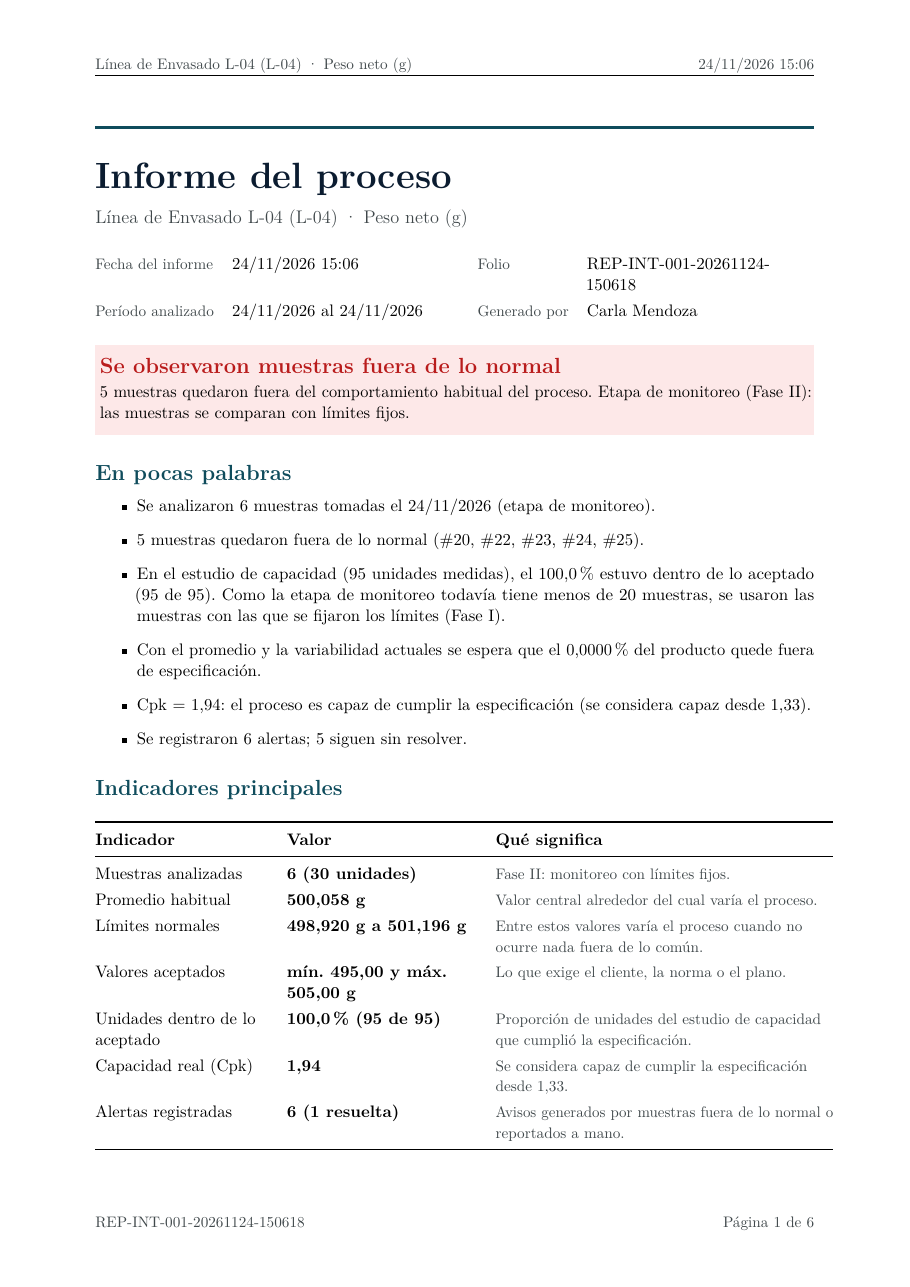
\includegraphics[width=0.48\linewidth]{img/informe_p1.png}\hfill
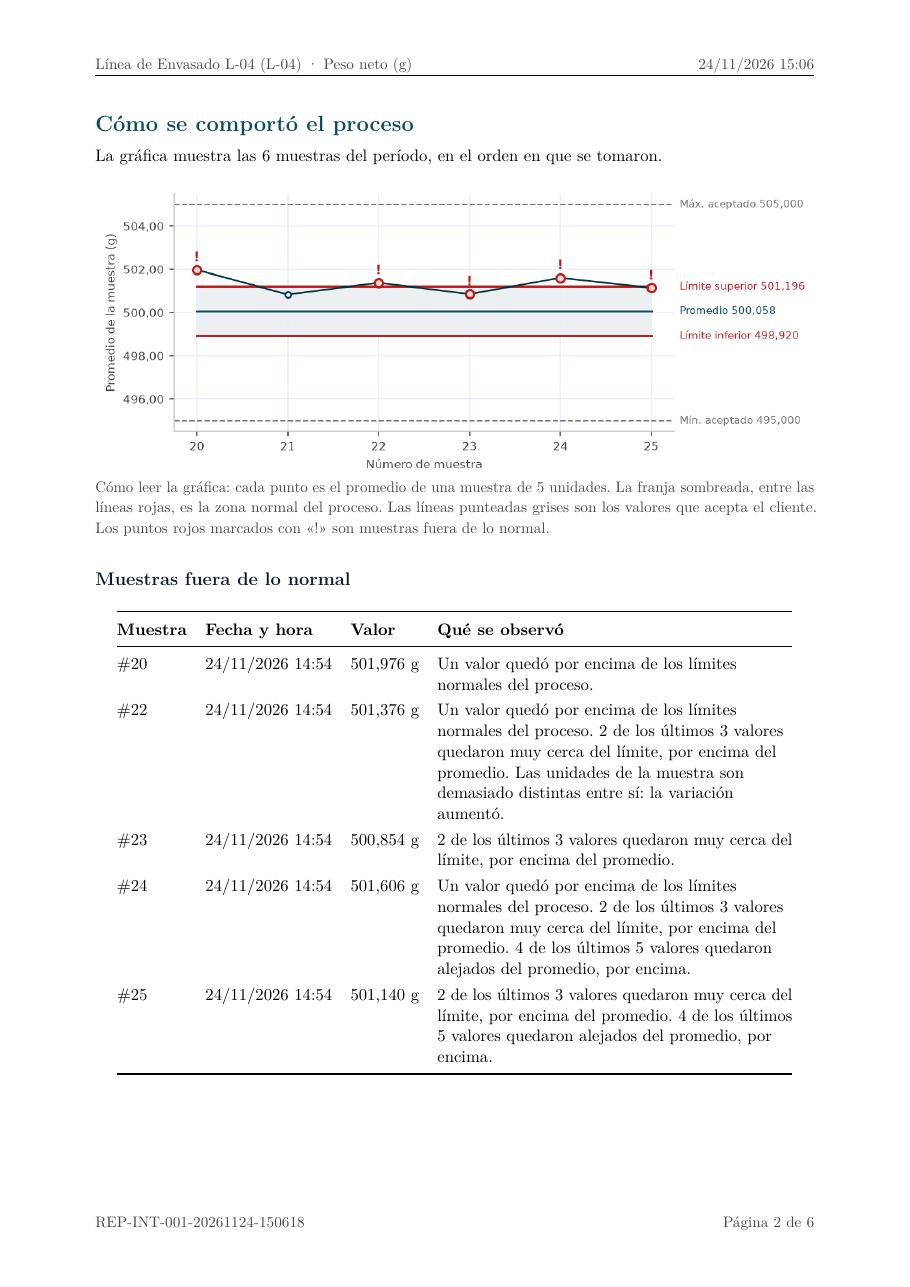
\includegraphics[width=0.48\linewidth]{img/informe_p2.png}
\caption{Primeras dos páginas del informe PDF generado con los datos de demostración.}
\end{figure}

Si el equipo no tiene LaTeX instalado, el PDF se genera con un formato alternativo con los mismos
textos, y la pantalla lo avisa. El \textbf{libro Excel} tiene una hoja por sección con los datos y
resultados numéricos.

\subsubsection{Historial y verificación}
La tabla \campo{Historial de Reportes Generados y Trazabilidad} lista los informes con su tipo,
formato, tamaño, fecha, autor y huella SHA-256. Desde ella se vuelven a descargar y se
\textbf{verifican}: la aplicación recalcula la huella del archivo guardado y confirma si fue
modificado después de generarse.

% ----------------------------------------------------------------------- 7.12
\subsection{Base de datos y respaldos}

\figura{ing_base_datos.png}{Pantalla Base de datos y respaldos.}{0.95}

\begin{itemize}
\item \textbf{Tus datos}: cuántos procesos, variables y muestras hay, dónde está la base, su tamaño
  y la versión del programa.
\item \boton{Respaldar ahora}: guarda una copia de la base en la carpeta de respaldos. Además, el
  programa hace una copia automática cada vez que se abre. Se conservan las últimas 20.
\item \boton{Descargar una copia}: guarda la base completa en un archivo \texttt{.db}, para
  archivarla o llevarla a otro computador.
\item \textbf{Respaldos}: la lista de copias con fecha, motivo y tamaño. Cada una se puede
  descargar o recuperar con \boton{Volver a este}.
\item \textbf{Restaurar desde un archivo}: con \boton{Elegir archivo .db} se reemplazan todos los
  datos por los de una copia descargada antes.
\item \boton{Cargar demostración}: solo con la base vacía.
\end{itemize}

\begin{cuidado}[Volver a un respaldo reemplaza todo]
Al restaurar, la base vuelve completa al estado de esa copia: se pierde todo lo registrado después,
en todos los procesos. Antes de hacerlo, la aplicación guarda automáticamente una copia de la base
actual, que aparece en la misma lista; así, la restauración siempre se puede deshacer.
\end{cuidado}

\textbf{Pasar los datos a otro computador:} en el equipo de origen, \boton{Descargar una copia}; en
el de destino, con CEP instalado, \boton{Elegir archivo .db} en \campo{Restaurar desde un archivo}.

% ======================================================================= 8
\section{Preguntas frecuentes y solución de problemas}

\begin{tabularx}{\linewidth}{@{}P{5.2cm}L@{}}
\toprule
\textbf{Situación} & \textbf{Qué hacer}\\
\midrule
Windows muestra \campo{Windows protegió su PC} al instalar. & Pulsar \boton{Más información} y \boton{Ejecutar de todas formas}. Aparece porque el instalador no tiene firma digital.\\
Subí la plantilla y las muestras de monitoreo no se cargaron. & Es lo esperado mientras la variable está en Fase I. Congelar los límites en Gráficos y volver a subir el mismo archivo.\\
Escribí mal un valor y ya guardé la muestra. & Durante 10 minutos, usar \boton{Deshacer} en Registrar muestra. Después de ese plazo, en Fase I el ingeniero puede excluirla con su causa.\\
Quiero cambiar el tipo de carta o el estimador de $\sigma$ y no me deja. & Solo se cambian en Fase I. Si los límites ya están congelados, primero \boton{Volver a Fase I} (con motivo).\\
No puedo eliminar una variable. & Solo se eliminan variables sin muestras, para no perder la trazabilidad.\\
Quiero quitar todo lo que cargué. & En Base de datos y respaldos, \boton{Volver a este} en un respaldo anterior a la carga. Ojo: afecta a todos los procesos.\\
La pantalla de supuestos rechaza la normalidad. & Revisar si los datos están redondeados (escalones en el gráfico Q-Q) y si son simétricos (ver la nota de la sección~\ref{sec:supuestos}).\\
El PDF dice que se usó el formato alternativo. & El equipo no tiene LaTeX. Instalar MiKTeX si se quiere el formato LaTeX; el contenido es el mismo.\\
La capacidad sale \campo{no confiable}. & El proceso tiene señales sin resolver. Atender las alertas o depurar la Fase I antes de interpretar los índices.\\
La próxima muestra aparece \campo{atrasada}. & Ya pasó el tiempo de la frecuencia definida desde la última muestra. Registrarla o revisar la frecuencia en el plan de muestreo.\\
¿Cómo sé si un informe fue modificado? & En Reportes, usar la verificación del historial: compara la huella SHA-256 del archivo con la registrada.\\
\bottomrule
\end{tabularx}

% ======================================================================= 9
\section{Glosario}\label{sec:glosario}
\begin{description}[leftmargin=1.5em,itemsep=0.25em,font=\bfseries]
\item[Alerta (alarma)] Aviso que genera la aplicación cuando una muestra cumple una regla de
  detección, o que crea una persona al reportar un problema.
\item[AOQ / AOQL] Calidad media de salida tras la inspección de lotes y su valor máximo.
\item[AQL] Nivel de calidad aceptable: la fracción defectuosa con la que un lote debería aceptarse
  casi siempre.
\item[ARL / ATS] Longitud media de corrida: cuántas muestras, en promedio, tarda la carta en dar
  una señal. El ATS es lo mismo expresado en tiempo.
\item[ATI] Inspección total media por lote.
\item[Causa asignable] Causa identificable de una variación anormal (un ajuste, un material, un
  error). Se opone a la \emph{causa común}, la variación natural del proceso.
\item[Cp, Cpk, Cpu, Cpl] Índices de capacidad: comparan la variación del proceso con la
  tolerancia. Cpk considera además dónde está el promedio.
\item[Fase I / Fase II] Etapa de estimación de los límites y etapa de monitoreo con los límites
  congelados.
\item[Fracción no conforme] Proporción de producto fuera de los valores aceptados, en porcentaje o
  en piezas por millón (ppm).
\item[LC, LCS, LCI] Línea central y límites de control superior e inferior.
\item[LES, LEI] Límites de especificación superior e inferior (valores aceptados).
\item[LTPD] Porcentaje defectuoso tolerable del lote: calidad que se quiere rechazar casi siempre.
\item[Muestra (subgrupo)] Grupo de unidades revisadas al mismo tiempo.
\item[p-valor] Probabilidad que usa una prueba estadística para decidir; si es menor que $\alpha$,
  se rechaza el supuesto.
\item[Reglas de Nelson y Western Electric] Conjuntos de patrones que indican que el proceso cambió
  (N1 a N8 y WE4).
\item[SHA-256] Huella digital de un archivo o de una configuración: cambia si se modifica
  cualquier dato.
\item[$\sigma$ (sigma)] Desviación estándar: mide cuánto varía el proceso.
\end{description}

\end{document}
